\documentclass{article}

\usepackage{graphicx}
\usepackage{listings}

\graphicspath{./}

\begin{document}
    \title  { \textbf{SYSC 4602 Assignment 6} }
    \author {
        David Song (101071234)\\
        Ghassan Arnouk (101078550)\\
        Zachary Porter (101069001)
    }

    \maketitle

    \clearpage
    \section*{Part 3: ARP request and reply}
    \begin{figure}[htbp]
        \centering
        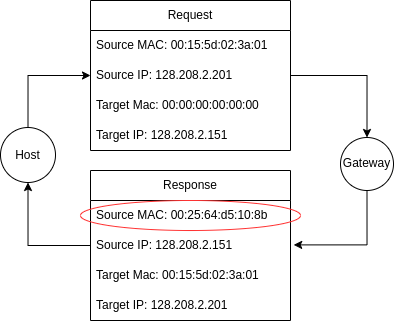
\includegraphics[width=\textwidth]{images/part3.drawio.png}
        \caption{ARP exchange}
    \end{figure}
    \clearpage
    \section*{Part 4: Details of ARP over Ethernet}
    \subsection*{1}
    \subsection*{2}
    \subsection*{3}
    \subsection*{4}
    \begin{enumerate}
        \item The opcode used to indicate a request is 1, and to indicate a reply is 2
        \item The ARP header size for a request is 28 bytes, and a reply is also 28 bytes
        \item The unknown MAC is listed as 00:00:00:00:00:00
        \item The value that indicates ARP layer in ethernet is 0x0806
        \item The reply is not brodcast, an is instead sent directly back to the sender of the request. This is shown in the trace
    \end{enumerate}}
    \subsection*{5}
\end{document}
